This chapter presents the hardware testbed. The assembled, setup system is
capable of dynamically adjusting its computational load relative to the on-site
energy production by photo-voltaic (PV) modules. Section
\ref{sec:hardware_components} lists all main physical components. Section
\ref{sec:hardware_assembly} shows the assembly of all components and explains
their interrelations. Subsequently section \ref{sec:software_setup} shows the
software setup, necessary to ensure functionality of the components, data
transmission and operability.  Section
\ref{sec:implementation_of_energy-aware_resource_management} presents the
implementation of Energy-Aware Resource Management for this testbed and
demonstrates the conformity with the requirements from section
\ref{sec:testbed_requirements}.

\section{Hardware Components}
\label{sec:hardware_components}

The testbed is mainly composed of the following hardware. As the compute node,
the single-board computer \emph{Raspberry Pi 3b+} serves as a viable choice due
to its low energy consumption, cost effectiveness and wide range of hardware
applications.\footnote{\url{https://raspberrypi.com}} Renewable energy is
produced by four PV modules, each generating 330 mA at 6 V as stated by its
manufacturer. Excess energy produced by the PV modules is stored in a 3.7 V,
6600 mAh lithium-ion polymer (LiPo) battery as backup energy source in case of
suboptimal solar conditions. Ultimately a component, connecting all components
listed above, is needed to measure the energy production of the PV modules and
the energy consumption of the compute node. \emph{SwitchDoc Labs} developed
\emph{SunControl}, an inexpensive solar power controller board, among multiple
other things capable of these tasks \cite{switchdoc_suncontrol} and is therefore
ideal for this testbed.

\section{Hardware Assembly}
\label{sec:hardware_assembly}

\section{Software Setup}
\label{sec:software_setup}

As the testbed is meant to be self-sufficient, remote communication is most
suitable for monitoring and operations. A Secure Shell (SSH) connection to the
Raspberry Pi is easily configured alongside the installation process of
Raspberry Pi OS Lite via their imager
software.\footnote{\url{https://raspberrypi.com/software/}} To enable
functionality of SunControl, installation of SwitchDoc's Python driver code
libraries are necessary. The official code from 2017 was written in Python
2.7.\footnote{\url{https://github.com/switchdoclabs/SDL_Pi_SunControl}} Since
Python 2 is deprecated since 2020 and vital official libraries are no longer
supported,\footnote{\url{https://python.org/doc/sunset-python-2/}} the codebase
needed to be refactored and ported from Python 2.7 to
3.7.\footnote{\url{https://github.com/marvin-steinke/SDL_Pi_SunControl}} To
allow SunControl to communicate with the Raspberry Pi, Inter-Integrated Circuit
(I$^2$C) support for the ARM core and Linux kernel need to be
enabled.\footnote{\label{footnote:config}\url{https://github.com/marvin-steinke/bachelors_thesis/blob/master/src/config/config.txt}}

\subsection{Energy Preservation}

The Raspberry Pi has many components, some of which might not be needed for the
specific use-cases of the testbed, but still make up a large portion of overall
energy consumption. The Bluetooth and HDMI module and the USB ports can be
disabled to preserve
energy.\footref{footnote:config}\footnote{\url{https://github.com/marvin-steinke/bachelors_thesis/blob/master/src/config/rc.local}}
Figure \ref{fig:idle} displays the idle power usage of the Raspberry Pi 3b+ over
the span of two minutes with the three components enabled and disabled
respectively. Enabling the components yields in an average energy consumption of
\mbox{2.1 W}, while disabling them results in an average consumption of just
\mbox{0.93 W}, preserving \mbox{1.17 W} in total. Since these components serve
no purpose in this version of the testbed, they are disabled in order to
preserve energy.

\begin{figure}[H]
    \centering
    \documentclass{standalone}
\usepackage{pgfplots}
\pgfplotsset{compat=1.18}

\begin{document}

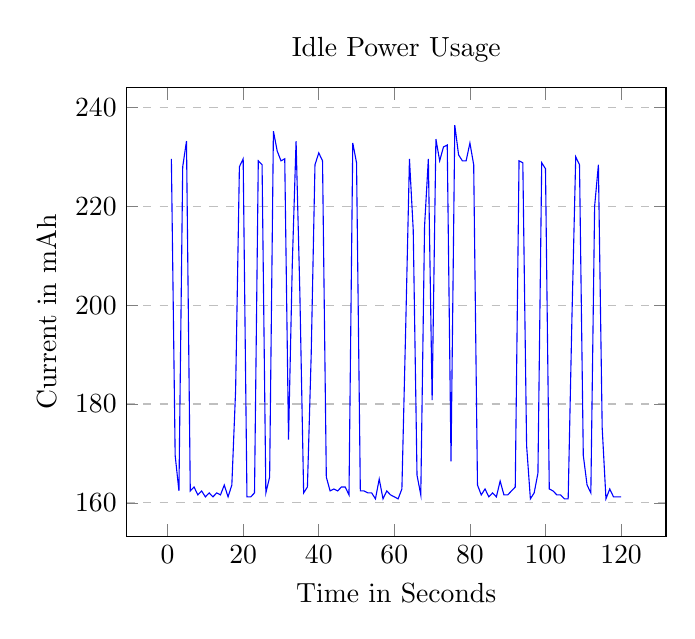
\begin{tikzpicture}
    \begin{axis}[
    title={Idle Power Usage},
    xlabel={Time in Seconds},
    ylabel={Current in mAh},
    %ytick=data,
    %xtick=data,
    ymajorgrids=true,
    legend pos=outer north east,
    grid style=dashed,
    ]
    \addplot[
        color=blue,
    ]
    coordinates {
        (1,229.60)
        (2,169.60)
        (3,162.40)
        (4,228.00)
        (5,233.20)
        (6,162.40)
        (7,163.20)
        (8,161.60)
        (9,162.40)
        (10,161.20)
        (11,162.00)
        (12,161.20)
        (13,162.00)
        (14,161.60)
        (15,163.60)
        (16,161.20)
        (17,163.60)
        (18,182.80)
        (19,228.00)
        (20,229.60)
        (21,161.20)
        (22,161.20)
        (23,162.00)
        (24,229.20)
        (25,228.40)
        (26,162.00)
        (27,165.20)
        (28,235.20)
        (29,231.20)
        (30,229.20)
        (31,229.60)
        (32,172.80)
        (33,208.40)
        (34,233.20)
        (35,202.40)
        (36,162.00)
        (37,163.20)
        (38,190.00)
        (39,228.40)
        (40,230.80)
        (41,229.20)
        (42,165.20)
        (43,162.40)
        (44,162.80)
        (45,162.40)
        (46,163.20)
        (47,163.20)
        (48,161.60)
        (49,232.80)
        (50,228.80)
        (51,162.40)
        (52,162.40)
        (53,162.00)
        (54,162.00)
        (55,160.80)
        (56,164.80)
        (57,160.80)
        (58,162.40)
        (59,161.60)
        (60,161.20)
        (61,160.80)
        (62,162.80)
        (63,195.20)
        (64,229.60)
        (65,215.20)
        (66,165.60)
        (67,161.60)
        (68,216.00)
        (69,229.60)
        (70,180.80)
        (71,233.60)
        (72,229.20)
        (73,232.00)
        (74,232.40)
        (75,168.40)
        (76,236.40)
        (77,230.40)
        (78,229.20)
        (79,229.20)
        (80,232.80)
        (81,228.40)
        (82,163.60)
        (83,161.60)
        (84,162.80)
        (85,161.20)
        (86,162.00)
        (87,161.20)
        (88,164.40)
        (89,161.60)
        (90,161.60)
        (91,162.40)
        (92,163.20)
        (93,229.20)
        (94,228.80)
        (95,171.60)
        (96,160.80)
        (97,162.00)
        (98,166.00)
        (99,228.80)
        (100,227.60)
        (101,162.80)
        (102,162.40)
        (103,161.60)
        (104,161.60)
        (105,160.80)
        (106,160.80)
        (107,197.60)
        (108,230.00)
        (109,228.40)
        (110,169.60)
        (111,163.60)
        (112,162.00)
        (113,220.00)
        (114,228.40)
        (115,175.20)
        (116,160.80)
        (117,162.80)
        (118,161.20)
        (119,161.20)
        (120,161.20)
    };
    \end{axis}
\end{tikzpicture}
mean: 186.32
\end{document}

    \caption{Idle power consumption with Bluetooth, HDMI and USB enabled and disabled}
    \label{fig:idle}
\end{figure}

\section{Implementation of Energy-Aware Resource Management}
\label{sec:implementation_of_energy-aware_resource_management}

Because the CPU is the main consumer of energy in the Raspberry Pi, scaling the
voltage and frequency of the CPU to control its consumption is the most viable
approach to control total energy consumption.
%the frequency and voltage of the Raspberry Pi's ARM CPU can be scaled
%dynamically with the \texttt{cpufreq}
%subsystem\footnote{\url{https://community.arm.com/oss-platforms/w/docs/528/cpufreq-dvfs}}.

\subsection{DVFS versus \texttt{cpulimit}}

\begin{figure}
    \centering
    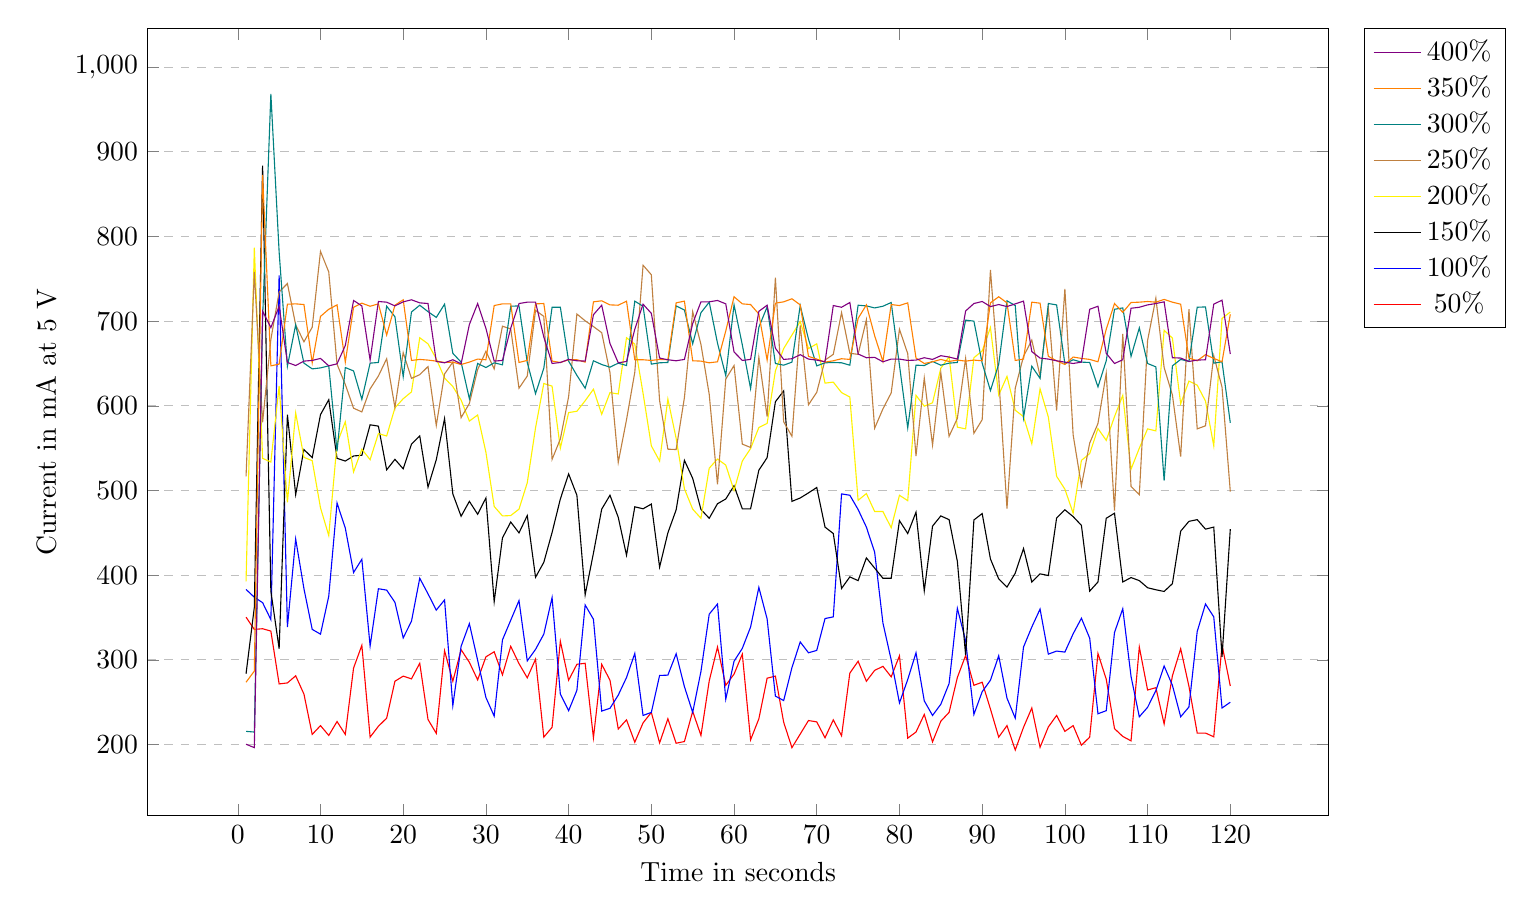
\begin{tikzpicture}
    \begin{axis}[
        xlabel={Time in seconds},
        ylabel={Current in mA at 5 V},
        %ytick=data,
        xtick={0,10,...,120},
        ymajorgrids=true,
        reverse legend,
        cycle list name=color list,
        legend pos=outer north east,
        grid style=dashed,
        height=10cm,
        width=15cm,
        scale only axis=true,
    ]
    \addplot
    coordinates {
        (1,350.40)
        (2,336.00)
        (3,336.80)
        (4,334.00)
        (5,271.60)
        (6,272.80)
        (7,281.20)
        (8,259.60)
        (9,212.00)
        (10,222.40)
        (11,210.80)
        (12,227.20)
        (13,212.00)
        (14,290.40)
        (15,317.20)
        (16,208.80)
        (17,221.60)
        (18,231.20)
        (19,274.80)
        (20,280.80)
        (21,277.60)
        (22,296.00)
        (23,229.60)
        (24,213.20)
        (25,310.80)
        (26,274.80)
        (27,312.00)
        (28,297.20)
        (29,276.40)
        (30,303.60)
        (31,309.60)
        (32,282.40)
        (33,316.00)
        (34,295.60)
        (35,278.80)
        (36,300.80)
        (37,208.80)
        (38,220.40)
        (39,322.00)
        (40,276.00)
        (41,294.80)
        (42,296.00)
        (43,208.00)
        (44,294.80)
        (45,276.00)
        (46,218.40)
        (47,229.20)
        (48,202.80)
        (49,225.60)
        (50,238.00)
        (51,202.00)
        (52,230.40)
        (53,201.60)
        (54,203.60)
        (55,239.20)
        (56,210.80)
        (57,275.20)
        (58,315.20)
        (59,270.00)
        (60,283.20)
        (61,306.80)
        (62,205.60)
        (63,230.40)
        (64,278.40)
        (65,280.80)
        (66,226.40)
        (67,196.40)
        (68,212.40)
        (69,228.40)
        (70,226.80)
        (71,208.00)
        (72,229.20)
        (73,210.40)
        (74,284.40)
        (75,298.40)
        (76,274.80)
        (77,287.60)
        (78,292.40)
        (79,280.00)
        (80,304.80)
        (81,207.60)
        (82,214.80)
        (83,235.60)
        (84,203.20)
        (85,227.60)
        (86,238.00)
        (87,279.20)
        (88,305.20)
        (89,270.00)
        (90,273.60)
        (91,242.00)
        (92,208.80)
        (93,222.40)
        (94,193.60)
        (95,220.40)
        (96,243.20)
        (97,196.80)
        (98,220.80)
        (99,234.40)
        (100,215.60)
        (101,222.40)
        (102,199.20)
        (103,208.80)
        (104,307.60)
        (105,277.20)
        (106,218.80)
        (107,209.60)
        (108,204.40)
        (109,315.20)
        (110,264.40)
        (111,267.20)
        (112,224.40)
        (113,281.20)
        (114,313.20)
        (115,268.80)
        (116,213.60)
        (117,213.60)
        (118,209.20)
        (119,317.60)
        (120,269.20)
    };
    \addlegendentry{50\%}
    \addplot
    coordinates {
        (1,383.20)
        (2,374.00)
        (3,367.60)
        (4,347.60)
        (5,754.00)
        (6,338.80)
        (7,442.80)
        (8,384.00)
        (9,336.00)
        (10,330.40)
        (11,375.20)
        (12,485.20)
        (13,455.60)
        (14,403.20)
        (15,418.80)
        (16,316.40)
        (17,384.00)
        (18,382.40)
        (19,368.00)
        (20,326.00)
        (21,345.60)
        (22,396.40)
        (23,378.00)
        (24,358.80)
        (25,370.80)
        (26,246.00)
        (27,316.00)
        (28,342.80)
        (29,299.60)
        (30,255.60)
        (31,233.60)
        (32,323.60)
        (33,346.80)
        (34,370.00)
        (35,298.80)
        (36,312.40)
        (37,330.40)
        (38,373.60)
        (39,259.60)
        (40,240.00)
        (41,264.00)
        (42,364.80)
        (43,348.00)
        (44,239.60)
        (45,242.80)
        (46,258.40)
        (47,279.20)
        (48,307.60)
        (49,234.40)
        (50,238.00)
        (51,281.60)
        (52,282.00)
        (53,307.20)
        (54,268.40)
        (55,238.00)
        (56,286.40)
        (57,354.00)
        (58,366.00)
        (59,253.60)
        (60,298.40)
        (61,313.60)
        (62,338.80)
        (63,385.60)
        (64,348.40)
        (65,257.20)
        (66,252.00)
        (67,290.80)
        (68,321.20)
        (69,308.40)
        (70,311.20)
        (71,348.80)
        (72,350.80)
        (73,496.00)
        (74,494.40)
        (75,477.60)
        (76,456.80)
        (77,427.20)
        (78,343.60)
        (79,300.00)
        (80,249.20)
        (81,276.80)
        (82,308.40)
        (83,251.60)
        (84,234.40)
        (85,247.60)
        (86,272.00)
        (87,360.80)
        (88,322.80)
        (89,235.60)
        (90,262.40)
        (91,276.00)
        (92,304.80)
        (93,254.80)
        (94,231.20)
        (95,315.20)
        (96,338.80)
        (97,360.00)
        (98,306.80)
        (99,310.40)
        (100,309.20)
        (101,330.80)
        (102,349.20)
        (103,325.60)
        (104,236.40)
        (105,240.00)
        (106,332.40)
        (107,360.40)
        (108,280.40)
        (109,232.80)
        (110,244.00)
        (111,263.60)
        (112,292.80)
        (113,270.00)
        (114,232.80)
        (115,244.40)
        (116,333.60)
        (117,366.00)
        (118,350.80)
        (119,243.20)
        (120,250.00)
    };
    \addlegendentry{100\%}
    \addplot
    coordinates {
        (1,283.60)
        (2,362.00)
        (3,883.60)
        (4,381.20)
        (5,313.20)
        (6,589.60)
        (7,495.20)
        (8,548.40)
        (9,538.80)
        (10,589.60)
        (11,607.20)
        (12,538.00)
        (13,534.80)
        (14,540.80)
        (15,541.60)
        (16,577.60)
        (17,576.00)
        (18,524.40)
        (19,536.80)
        (20,525.60)
        (21,554.80)
        (22,564.40)
        (23,504.00)
        (24,536.40)
        (25,584.80)
        (26,496.00)
        (27,469.60)
        (28,487.20)
        (29,472.00)
        (30,491.20)
        (31,368.80)
        (32,444.00)
        (33,462.80)
        (34,450.00)
        (35,470.40)
        (36,397.60)
        (37,415.20)
        (38,450.40)
        (39,490.00)
        (40,519.60)
        (41,494.40)
        (42,376.80)
        (43,426.00)
        (44,478.00)
        (45,494.40)
        (46,468.40)
        (47,423.60)
        (48,480.80)
        (49,478.40)
        (50,484.00)
        (51,409.60)
        (52,450.00)
        (53,477.20)
        (54,535.60)
        (55,514.40)
        (56,477.60)
        (57,467.20)
        (58,484.40)
        (59,490.00)
        (60,505.60)
        (61,478.40)
        (62,478.40)
        (63,524.00)
        (64,538.80)
        (65,604.80)
        (66,617.60)
        (67,487.20)
        (68,491.20)
        (69,497.20)
        (70,503.60)
        (71,456.80)
        (72,449.20)
        (73,384.40)
        (74,398.00)
        (75,393.60)
        (76,420.40)
        (77,408.40)
        (78,396.40)
        (79,396.40)
        (80,464.40)
        (81,449.20)
        (82,474.40)
        (83,381.60)
        (84,458.00)
        (85,470.00)
        (86,465.60)
        (87,416.40)
        (88,305.60)
        (89,465.20)
        (90,472.80)
        (91,419.20)
        (92,395.60)
        (93,386.00)
        (94,402.40)
        (95,431.60)
        (96,392.00)
        (97,401.60)
        (98,399.60)
        (99,467.60)
        (100,477.20)
        (101,469.20)
        (102,458.80)
        (103,381.20)
        (104,392.00)
        (105,467.20)
        (106,473.20)
        (107,392.00)
        (108,397.20)
        (109,393.60)
        (110,385.20)
        (111,382.80)
        (112,380.80)
        (113,390.00)
        (114,452.00)
        (115,463.60)
        (116,465.60)
        (117,454.40)
        (118,456.80)
        (119,303.60)
        (120,454.40)
    };
    \addlegendentry{150\%}
    \addplot
    coordinates {
        (1,392.80)
        (2,786.80)
        (3,538.00)
        (4,533.60)
        (5,623.60)
        (6,486.00)
        (7,591.60)
        (8,539.20)
        (9,535.20)
        (10,479.60)
        (11,446.80)
        (12,555.60)
        (13,581.20)
        (14,522.00)
        (15,548.80)
        (16,536.40)
        (17,567.20)
        (18,564.40)
        (19,597.60)
        (20,608.40)
        (21,616.40)
        (22,680.40)
        (23,673.20)
        (24,655.60)
        (25,632.80)
        (26,622.80)
        (27,606.80)
        (28,582.00)
        (29,589.20)
        (30,545.20)
        (31,481.20)
        (32,470.00)
        (33,470.40)
        (34,478.00)
        (35,509.20)
        (36,574.00)
        (37,626.40)
        (38,623.20)
        (39,550.00)
        (40,592.00)
        (41,593.60)
        (42,606.00)
        (43,619.60)
        (44,590.00)
        (45,615.60)
        (46,614.00)
        (47,680.40)
        (48,672.80)
        (49,614.80)
        (50,552.80)
        (51,534.80)
        (52,608.00)
        (53,561.60)
        (54,502.00)
        (55,478.00)
        (56,467.20)
        (57,526.40)
        (58,537.20)
        (59,530.00)
        (60,500.00)
        (61,534.80)
        (62,549.60)
        (63,574.40)
        (64,579.20)
        (65,641.20)
        (66,667.60)
        (67,683.60)
        (68,699.60)
        (69,667.60)
        (70,673.20)
        (71,626.80)
        (72,628.00)
        (73,615.60)
        (74,610.40)
        (75,488.40)
        (76,496.40)
        (77,475.20)
        (78,475.20)
        (79,456.00)
        (80,494.40)
        (81,488.00)
        (82,612.40)
        (83,599.60)
        (84,603.60)
        (85,644.40)
        (86,658.00)
        (87,574.80)
        (88,572.80)
        (89,656.80)
        (90,664.80)
        (91,692.40)
        (92,612.80)
        (93,634.80)
        (94,594.80)
        (95,587.20)
        (96,555.20)
        (97,620.00)
        (98,586.80)
        (99,516.80)
        (100,501.60)
        (101,473.20)
        (102,535.60)
        (103,543.60)
        (104,573.20)
        (105,559.20)
        (106,587.20)
        (107,612.40)
        (108,525.20)
        (109,550.00)
        (110,572.80)
        (111,570.40)
        (112,689.20)
        (113,680.00)
        (114,602.40)
        (115,629.20)
        (116,624.40)
        (117,605.60)
        (118,552.80)
        (119,703.20)
        (120,710.80)
    };
    \addlegendentry{200\%}
    \addplot
    coordinates {
        (1,516.80)
        (2,758.00)
        (3,580.40)
        (4,678.40)
        (5,734.40)
        (6,744.40)
        (7,695.60)
        (8,675.60)
        (9,692.80)
        (10,782.40)
        (11,758.00)
        (12,649.20)
        (13,625.20)
        (14,597.20)
        (15,592.80)
        (16,620.00)
        (17,635.20)
        (18,655.60)
        (19,598.00)
        (20,662.80)
        (21,632.40)
        (22,636.80)
        (23,646.40)
        (24,576.80)
        (25,637.60)
        (26,651.60)
        (27,586.00)
        (28,602.80)
        (29,642.80)
        (30,664.40)
        (31,643.60)
        (32,694.00)
        (33,690.80)
        (34,620.80)
        (35,635.20)
        (36,712.80)
        (37,705.60)
        (38,536.80)
        (39,560.80)
        (40,610.80)
        (41,708.40)
        (42,700.40)
        (43,693.60)
        (44,686.40)
        (45,639.20)
        (46,533.20)
        (47,583.60)
        (48,639.60)
        (49,766.00)
        (50,754.80)
        (51,606.00)
        (52,548.80)
        (53,548.40)
        (54,609.60)
        (55,711.20)
        (56,672.40)
        (57,613.60)
        (58,507.20)
        (59,631.60)
        (60,647.60)
        (61,554.80)
        (62,550.80)
        (63,657.20)
        (64,587.20)
        (65,751.20)
        (66,581.20)
        (67,564.00)
        (68,694.80)
        (69,601.20)
        (70,616.00)
        (71,654.00)
        (72,660.80)
        (73,710.00)
        (74,662.00)
        (75,660.80)
        (76,701.60)
        (77,573.60)
        (78,596.40)
        (79,615.20)
        (80,690.40)
        (81,661.60)
        (82,540.80)
        (83,632.80)
        (84,553.60)
        (85,639.20)
        (86,564.00)
        (87,585.20)
        (88,656.00)
        (89,567.60)
        (90,583.60)
        (91,760.40)
        (92,634.00)
        (93,478.80)
        (94,620.80)
        (95,658.40)
        (96,677.60)
        (97,635.20)
        (98,715.60)
        (99,594.40)
        (100,738.00)
        (101,565.60)
        (102,505.60)
        (103,556.00)
        (104,579.20)
        (105,638.40)
        (106,476.40)
        (107,684.80)
        (108,504.80)
        (109,495.20)
        (110,677.20)
        (111,727.20)
        (112,645.20)
        (113,612.80)
        (114,540.00)
        (115,714.00)
        (116,572.80)
        (117,576.40)
        (118,659.20)
        (119,622.00)
        (120,498.80)
    };
    \addlegendentry{250\%}
    \addplot
    coordinates {
        (1,215.60)
        (2,214.80)
        (3,702.40)
        (4,968.40)
        (5,781.60)
        (6,646.80)
        (7,695.60)
        (8,650.40)
        (9,643.60)
        (10,644.80)
        (11,647.20)
        (12,546.40)
        (13,645.20)
        (14,641.20)
        (15,607.60)
        (16,650.40)
        (17,651.20)
        (18,717.60)
        (19,705.20)
        (20,634.40)
        (21,710.80)
        (22,718.80)
        (23,711.20)
        (24,704.40)
        (25,720.00)
        (26,662.00)
        (27,651.60)
        (28,608.40)
        (29,650.00)
        (30,645.20)
        (31,650.80)
        (32,648.40)
        (33,717.60)
        (34,718.00)
        (35,651.20)
        (36,614.40)
        (37,644.40)
        (38,716.40)
        (39,716.40)
        (40,652.80)
        (41,636.00)
        (42,620.80)
        (43,653.20)
        (44,648.80)
        (45,645.60)
        (46,650.40)
        (47,647.60)
        (48,723.60)
        (49,717.60)
        (50,649.20)
        (51,650.80)
        (52,651.20)
        (53,718.00)
        (54,713.20)
        (55,673.20)
        (56,710.00)
        (57,722.40)
        (58,674.00)
        (59,635.60)
        (60,719.20)
        (61,672.00)
        (62,620.40)
        (63,692.80)
        (64,716.80)
        (65,650.00)
        (66,648.00)
        (67,651.60)
        (68,718.40)
        (69,678.80)
        (70,647.20)
        (71,650.80)
        (72,651.20)
        (73,650.80)
        (74,648.00)
        (75,718.80)
        (76,718.00)
        (77,715.60)
        (78,717.60)
        (79,722.00)
        (80,648.00)
        (81,574.00)
        (82,648.00)
        (83,647.60)
        (84,652.40)
        (85,648.00)
        (86,650.40)
        (87,651.20)
        (88,701.20)
        (89,700.00)
        (90,650.40)
        (91,618.00)
        (92,649.20)
        (93,724.00)
        (94,718.40)
        (95,586.00)
        (96,646.80)
        (97,632.40)
        (98,720.80)
        (99,719.20)
        (100,649.60)
        (101,654.40)
        (102,651.60)
        (103,651.20)
        (104,622.40)
        (105,653.20)
        (106,714.00)
        (107,715.60)
        (108,658.40)
        (109,692.00)
        (110,650.00)
        (111,646.00)
        (112,511.60)
        (113,647.20)
        (114,654.80)
        (115,652.40)
        (116,716.40)
        (117,716.80)
        (118,650.40)
        (119,652.00)
        (120,580.00)
    };
    \addlegendentry{300\%}
    \addplot
    coordinates {
        (1,273.60)
        (2,286.80)
        (3,872.80)
        (4,647.20)
        (5,649.20)
        (6,720.00)
        (7,720.40)
        (8,719.60)
        (9,650.80)
        (10,705.60)
        (11,714.00)
        (12,719.20)
        (13,651.60)
        (14,716.40)
        (15,721.20)
        (16,717.60)
        (17,720.40)
        (18,683.60)
        (19,718.80)
        (20,725.20)
        (21,653.60)
        (22,654.80)
        (23,654.00)
        (24,652.80)
        (25,651.20)
        (26,651.60)
        (27,648.80)
        (28,651.60)
        (29,655.20)
        (30,654.40)
        (31,718.40)
        (32,720.40)
        (33,720.40)
        (34,651.20)
        (35,653.60)
        (36,720.40)
        (37,720.80)
        (38,652.80)
        (39,651.20)
        (40,654.40)
        (41,654.40)
        (42,651.60)
        (43,722.80)
        (44,724.00)
        (45,719.20)
        (46,718.80)
        (47,723.60)
        (48,654.40)
        (49,654.40)
        (50,653.60)
        (51,654.80)
        (52,654.40)
        (53,721.60)
        (54,723.60)
        (55,653.20)
        (56,652.80)
        (57,650.80)
        (58,652.00)
        (59,688.40)
        (60,728.80)
        (61,720.40)
        (62,719.60)
        (63,708.40)
        (64,654.00)
        (65,721.20)
        (66,722.80)
        (67,726.40)
        (68,719.20)
        (69,658.40)
        (70,655.20)
        (71,651.60)
        (72,653.20)
        (73,655.60)
        (74,654.80)
        (75,703.20)
        (76,719.20)
        (77,682.80)
        (78,652.40)
        (79,719.60)
        (80,718.40)
        (81,721.60)
        (82,656.40)
        (83,650.00)
        (84,652.00)
        (85,654.80)
        (86,652.40)
        (87,654.00)
        (88,652.80)
        (89,654.00)
        (90,653.20)
        (91,721.60)
        (92,728.80)
        (93,721.60)
        (94,653.60)
        (95,655.20)
        (96,722.40)
        (97,721.20)
        (98,658.40)
        (99,653.20)
        (100,648.80)
        (101,657.60)
        (102,656.00)
        (103,654.80)
        (104,652.00)
        (105,690.40)
        (106,720.80)
        (107,710.40)
        (108,722.00)
        (109,722.40)
        (110,723.20)
        (111,722.40)
        (112,725.60)
        (113,722.40)
        (114,720.00)
        (115,656.40)
        (116,653.20)
        (117,660.40)
        (118,656.00)
        (119,652.00)
        (120,708.00)
    };
    \addlegendentry{350\%}
    \addplot
    coordinates {
        (1,200.40)
        (2,196.40)
        (3,712.00)
        (4,692.40)
        (5,717.60)
        (6,651.20)
        (7,647.60)
        (8,652.80)
        (9,653.60)
        (10,656.00)
        (11,647.20)
        (12,649.60)
        (13,671.20)
        (14,724.40)
        (15,718.00)
        (16,654.00)
        (17,723.20)
        (18,722.40)
        (19,718.00)
        (20,722.80)
        (21,725.20)
        (22,721.60)
        (23,720.80)
        (24,652.40)
        (25,650.80)
        (26,654.40)
        (27,649.60)
        (28,696.00)
        (29,720.80)
        (30,691.60)
        (31,652.80)
        (32,653.60)
        (33,691.60)
        (34,720.80)
        (35,722.40)
        (36,722.40)
        (37,681.20)
        (38,650.00)
        (39,651.20)
        (40,654.80)
        (41,653.20)
        (42,652.80)
        (43,707.60)
        (44,718.80)
        (45,673.60)
        (46,650.80)
        (47,652.40)
        (48,690.40)
        (49,720.00)
        (50,709.20)
        (51,656.40)
        (52,654.40)
        (53,653.20)
        (54,654.80)
        (55,697.20)
        (56,722.80)
        (57,722.80)
        (58,724.40)
        (59,720.40)
        (60,663.60)
        (61,653.60)
        (62,654.80)
        (63,711.60)
        (64,718.80)
        (65,668.00)
        (66,654.80)
        (67,655.60)
        (68,660.40)
        (69,655.20)
        (70,654.00)
        (71,652.00)
        (72,718.40)
        (73,716.40)
        (74,722.00)
        (75,661.20)
        (76,656.80)
        (77,657.20)
        (78,652.00)
        (79,655.20)
        (80,655.20)
        (81,653.60)
        (82,654.00)
        (83,656.80)
        (84,654.80)
        (85,659.20)
        (86,657.60)
        (87,655.20)
        (88,712.00)
        (89,720.80)
        (90,723.20)
        (91,717.20)
        (92,719.60)
        (93,717.20)
        (94,720.40)
        (95,723.60)
        (96,664.00)
        (97,656.40)
        (98,655.20)
        (99,653.20)
        (100,651.60)
        (101,650.00)
        (102,651.60)
        (103,714.00)
        (104,717.60)
        (105,662.00)
        (106,650.00)
        (107,654.40)
        (108,715.20)
        (109,716.40)
        (110,719.20)
        (111,720.80)
        (112,722.80)
        (113,656.80)
        (114,656.40)
        (115,652.40)
        (116,654.00)
        (117,654.40)
        (118,720.00)
        (119,724.80)
        (120,661.20)
    };
    \addlegendentry{400\%}
    \end{axis}
\end{tikzpicture}

    \caption{Power usage under load with \texttt{cpulimit}}
    \label{fig:cpulimit_load}
\end{figure}

\begin{figure}
    \centering
    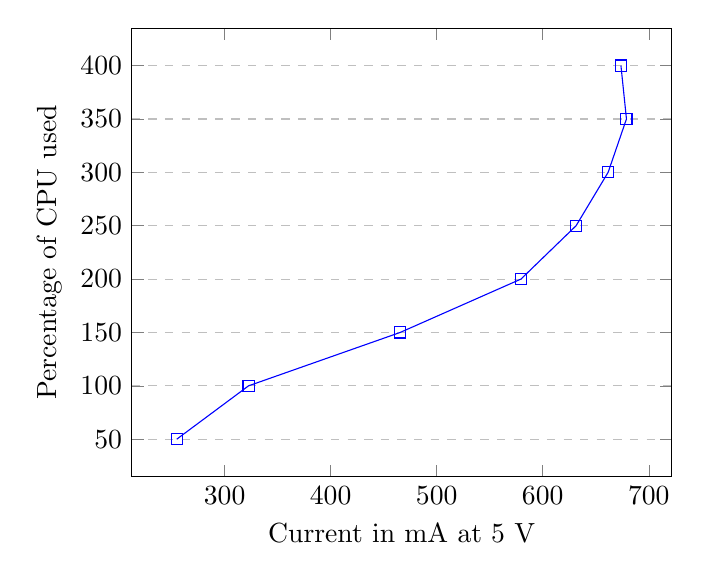
\begin{tikzpicture}
    \begin{axis}[
        xlabel={Current in mA at 5 V},
        ylabel={Percentage of CPU used},
        ytick=data,
        %xtick=data,
        ymajorgrids=true,
        grid style=dashed,
        cycle list name=color list,
    ]
    \addplot[
        mark=square,
        color=blue,
    ]
    coordinates {
        (254.90,50)
        (322.62,100)
        (465.57,150)
        (579.45,200)
        (631.46,250)
        (661.65,300)
        (678.93,350)
        (673.72,400)
    };
    \end{axis}
\end{tikzpicture}

    \caption{Mean power usage under load with \texttt{cpulimit}}
    \label{fig:cpulimit_mean}
\end{figure}

\begin{figure}
    \centering
    \documentclass{standalone}
\usepackage{pgfplots}
\pgfplotsset{compat=1.18}

\begin{document}

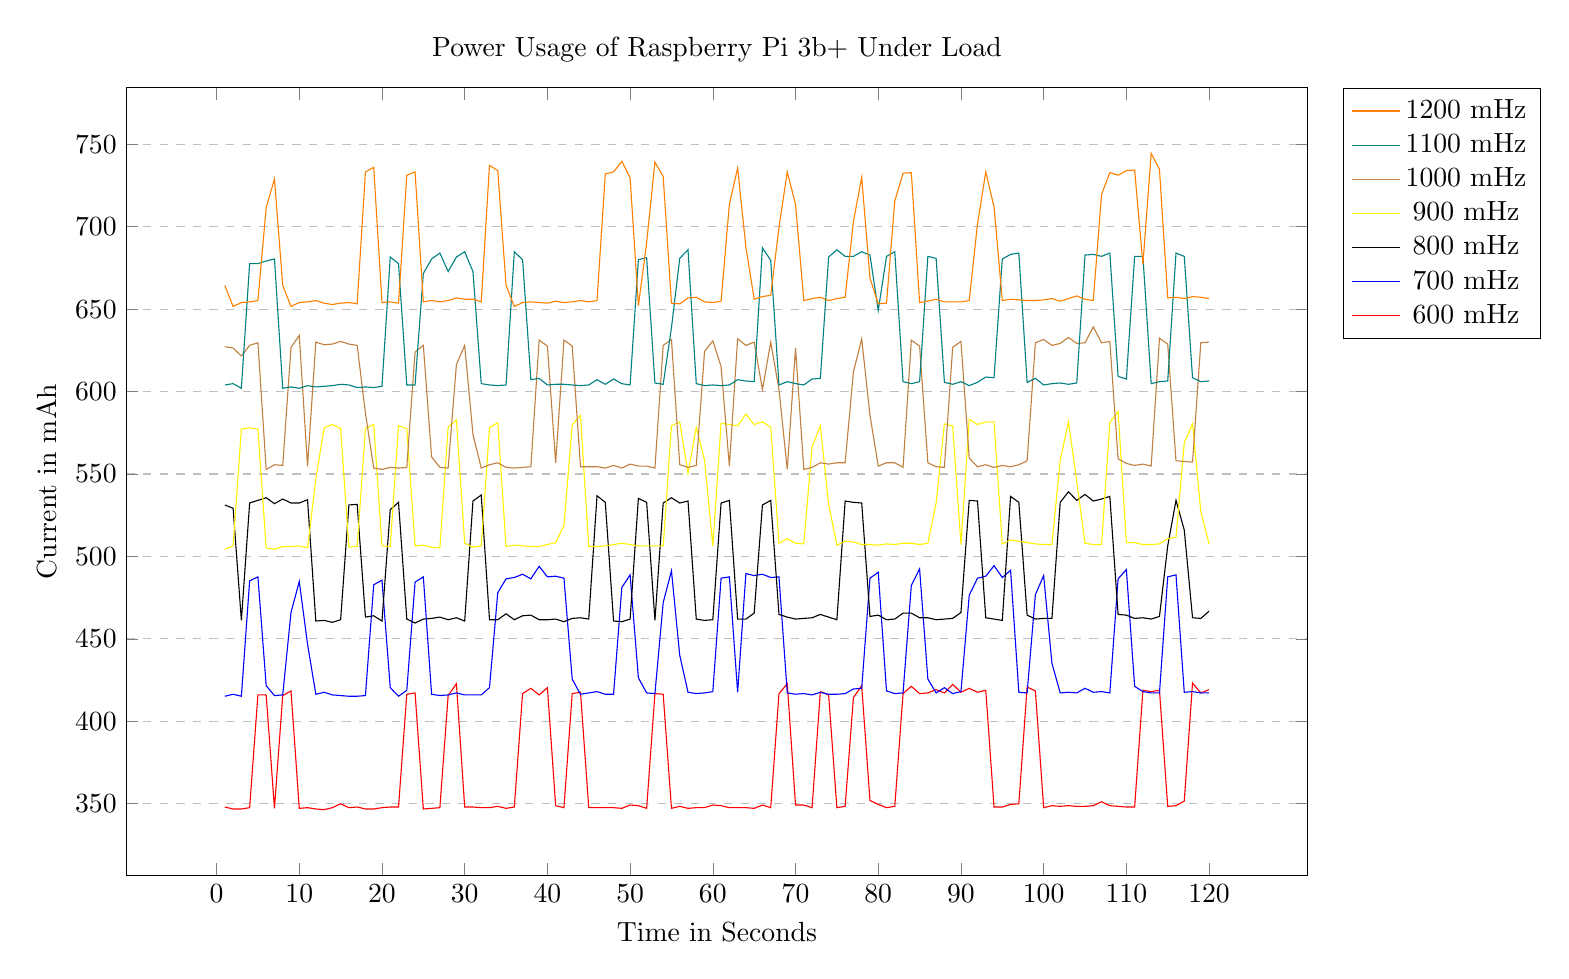
\begin{tikzpicture}
    \begin{axis}[
        title={Power Usage of Raspberry Pi 3b+ Under Load},
        xlabel={Time in Seconds},
        ylabel={Current in mAh},
        %ytick=data,
        xtick={0,10,...,120},
        ymajorgrids=true,
        reverse legend,
        cycle list name=color list,
        legend pos=outer north east,
        grid style=dashed,
        height=10cm,
        width=15cm,
        scale only axis=true,
    ]
    \addplot
    coordinates {
        (1,348.00)
        (2,346.80)
        (3,346.80)
        (4,347.60)
        (5,416.00)
        (6,416.00)
        (7,347.20)
        (8,415.60)
        (9,418.40)
        (10,347.20)
        (11,347.60)
        (12,346.80)
        (13,346.40)
        (14,347.60)
        (15,350.00)
        (16,347.60)
        (17,348.00)
        (18,346.80)
        (19,346.80)
        (20,347.60)
        (21,348.00)
        (22,348.00)
        (23,416.40)
        (24,417.20)
        (25,346.80)
        (26,347.20)
        (27,347.60)
        (28,415.60)
        (29,422.80)
        (30,348.00)
        (31,348.00)
        (32,347.60)
        (33,347.60)
        (34,348.40)
        (35,347.20)
        (36,348.00)
        (37,416.80)
        (38,420.00)
        (39,416.00)
        (40,420.40)
        (41,348.80)
        (42,347.60)
        (43,416.80)
        (44,417.60)
        (45,347.60)
        (46,347.60)
        (47,347.60)
        (48,347.60)
        (49,347.20)
        (50,349.20)
        (51,348.80)
        (52,347.20)
        (53,416.80)
        (54,416.40)
        (55,347.20)
        (56,348.40)
        (57,347.20)
        (58,347.60)
        (59,347.60)
        (60,349.20)
        (61,348.80)
        (62,347.60)
        (63,347.60)
        (64,347.60)
        (65,347.20)
        (66,349.20)
        (67,347.60)
        (68,416.80)
        (69,422.80)
        (70,349.20)
        (71,349.20)
        (72,347.60)
        (73,418.00)
        (74,416.00)
        (75,347.60)
        (76,348.40)
        (77,414.40)
        (78,421.60)
        (79,352.00)
        (80,349.60)
        (81,347.60)
        (82,348.40)
        (83,416.80)
        (84,421.20)
        (85,416.80)
        (86,417.20)
        (87,419.20)
        (88,417.20)
        (89,422.40)
        (90,417.60)
        (91,420.00)
        (92,417.60)
        (93,418.80)
        (94,348.00)
        (95,348.00)
        (96,349.60)
        (97,350.00)
        (98,420.80)
        (99,418.40)
        (100,347.60)
        (101,348.80)
        (102,348.40)
        (103,348.80)
        (104,348.40)
        (105,348.40)
        (106,348.80)
        (107,351.20)
        (108,348.80)
        (109,348.40)
        (110,348.00)
        (111,348.00)
        (112,418.80)
        (113,418.00)
        (114,418.80)
        (115,348.40)
        (116,348.80)
        (117,351.60)
        (118,423.20)
        (119,417.20)
        (120,419.20)
    };
    \addlegendentry{600 mHz} % 372.07
    \addplot
    coordinates {
        (1,415.20)
        (2,416.40)
        (3,415.20)
        (4,485.20)
        (5,487.60)
        (6,421.60)
        (7,415.60)
        (8,416.00)
        (9,466.00)
        (10,484.80)
        (11,446.80)
        (12,416.40)
        (13,417.60)
        (14,416.00)
        (15,415.60)
        (16,415.20)
        (17,415.20)
        (18,415.60)
        (19,482.80)
        (20,485.60)
        (21,420.40)
        (22,415.20)
        (23,418.80)
        (24,484.40)
        (25,487.60)
        (26,416.40)
        (27,415.60)
        (28,416.00)
        (29,417.20)
        (30,416.00)
        (31,416.00)
        (32,416.00)
        (33,420.40)
        (34,478.00)
        (35,486.40)
        (36,487.20)
        (37,489.20)
        (38,486.40)
        (39,494.00)
        (40,487.60)
        (41,488.00)
        (42,486.80)
        (43,425.60)
        (44,416.40)
        (45,417.20)
        (46,418.00)
        (47,416.40)
        (48,416.40)
        (49,481.20)
        (50,488.80)
        (51,426.40)
        (52,417.20)
        (53,416.80)
        (54,472.00)
        (55,491.20)
        (56,440.00)
        (57,417.60)
        (58,416.80)
        (59,417.20)
        (60,418.00)
        (61,486.80)
        (62,487.60)
        (63,417.60)
        (64,489.60)
        (65,488.40)
        (66,489.20)
        (67,487.20)
        (68,487.60)
        (69,417.20)
        (70,416.40)
        (71,416.80)
        (72,416.00)
        (73,417.60)
        (74,416.40)
        (75,416.40)
        (76,416.80)
        (77,419.60)
        (78,420.00)
        (79,486.80)
        (80,490.40)
        (81,418.40)
        (82,416.80)
        (83,417.20)
        (84,482.40)
        (85,492.40)
        (86,425.60)
        (87,417.20)
        (88,420.40)
        (89,416.80)
        (90,418.00)
        (91,476.40)
        (92,486.80)
        (93,488.00)
        (94,494.40)
        (95,487.20)
        (96,491.60)
        (97,417.60)
        (98,417.20)
        (99,476.80)
        (100,488.40)
        (101,435.20)
        (102,417.20)
        (103,417.60)
        (104,417.20)
        (105,420.00)
        (106,417.60)
        (107,418.00)
        (108,417.20)
        (109,486.40)
        (110,492.00)
        (111,421.20)
        (112,418.00)
        (113,417.20)
        (114,417.20)
        (115,487.60)
        (116,488.80)
        (117,417.60)
        (118,418.00)
        (119,417.20)
        (120,417.20)
    };
    \addlegendentry{700 mHz} % 443.33
    \addplot
    coordinates {
        (1,531.20)
        (2,529.20)
        (3,461.20)
        (4,532.40)
        (5,534.00)
        (6,535.60)
        (7,532.00)
        (8,534.80)
        (9,532.40)
        (10,532.40)
        (11,534.40)
        (12,460.80)
        (13,461.20)
        (14,460.00)
        (15,461.60)
        (16,531.20)
        (17,531.60)
        (18,463.20)
        (19,464.00)
        (20,460.80)
        (21,528.40)
        (22,532.80)
        (23,462.00)
        (24,459.60)
        (25,462.00)
        (26,462.40)
        (27,463.20)
        (28,461.60)
        (29,462.80)
        (30,460.80)
        (31,533.60)
        (32,537.20)
        (33,461.60)
        (34,461.60)
        (35,465.20)
        (36,461.60)
        (37,464.00)
        (38,464.40)
        (39,461.60)
        (40,461.60)
        (41,462.00)
        (42,460.40)
        (43,462.40)
        (44,462.80)
        (45,462.00)
        (46,536.80)
        (47,532.80)
        (48,460.80)
        (49,460.40)
        (50,462.00)
        (51,535.20)
        (52,532.80)
        (53,461.20)
        (54,532.40)
        (55,535.60)
        (56,532.40)
        (57,533.60)
        (58,462.00)
        (59,461.20)
        (60,461.60)
        (61,532.40)
        (62,534.00)
        (63,462.00)
        (64,462.00)
        (65,465.60)
        (66,531.20)
        (67,534.00)
        (68,464.80)
        (69,463.20)
        (70,462.00)
        (71,462.40)
        (72,462.80)
        (73,464.80)
        (74,463.20)
        (75,461.60)
        (76,533.60)
        (77,532.80)
        (78,532.40)
        (79,463.60)
        (80,464.40)
        (81,461.60)
        (82,462.00)
        (83,465.60)
        (84,465.60)
        (85,462.80)
        (86,462.80)
        (87,461.60)
        (88,462.00)
        (89,462.40)
        (90,466.00)
        (91,534.00)
        (92,533.60)
        (93,462.80)
        (94,462.00)
        (95,461.20)
        (96,536.40)
        (97,532.80)
        (98,464.40)
        (99,462.00)
        (100,462.40)
        (101,462.40)
        (102,532.80)
        (103,539.20)
        (104,534.00)
        (105,537.60)
        (106,533.60)
        (107,534.80)
        (108,536.40)
        (109,464.80)
        (110,464.40)
        (111,462.40)
        (112,462.80)
        (113,462.00)
        (114,463.60)
        (115,506.40)
        (116,534.00)
        (117,516.00)
        (118,462.80)
        (119,462.40)
        (120,466.80)
    };
    \addlegendentry{800 mHz} % 488.82
    \addplot
    coordinates {
        (1,504.40)
        (2,506.40)
        (3,577.20)
        (4,578.00)
        (5,577.20)
        (6,505.20)
        (7,504.40)
        (8,506.00)
        (9,506.00)
        (10,506.40)
        (11,505.20)
        (12,546.80)
        (13,578.00)
        (14,580.00)
        (15,577.60)
        (16,505.60)
        (17,506.00)
        (18,577.60)
        (19,580.00)
        (20,506.40)
        (21,506.00)
        (22,579.20)
        (23,577.60)
        (24,506.40)
        (25,506.80)
        (26,505.60)
        (27,505.20)
        (28,578.40)
        (29,582.80)
        (30,508.00)
        (31,505.60)
        (32,506.40)
        (33,578.00)
        (34,581.20)
        (35,506.00)
        (36,506.80)
        (37,506.40)
        (38,506.00)
        (39,506.00)
        (40,507.20)
        (41,508.40)
        (42,518.80)
        (43,579.60)
        (44,585.60)
        (45,506.00)
        (46,506.00)
        (47,506.40)
        (48,507.20)
        (49,508.00)
        (50,507.20)
        (51,506.40)
        (52,506.40)
        (53,506.40)
        (54,506.40)
        (55,579.20)
        (56,581.60)
        (57,550.40)
        (58,578.40)
        (59,558.40)
        (60,506.40)
        (61,580.80)
        (62,580.00)
        (63,579.20)
        (64,586.40)
        (65,580.00)
        (66,581.60)
        (67,578.40)
        (68,508.00)
        (69,510.80)
        (70,508.00)
        (71,507.60)
        (72,566.40)
        (73,579.20)
        (74,531.60)
        (75,506.80)
        (76,509.20)
        (77,508.80)
        (78,507.20)
        (79,507.20)
        (80,506.80)
        (81,507.60)
        (82,507.20)
        (83,508.00)
        (84,508.00)
        (85,507.20)
        (86,508.00)
        (87,532.40)
        (88,580.40)
        (89,579.20)
        (90,507.20)
        (91,583.20)
        (92,580.00)
        (93,581.60)
        (94,581.60)
        (95,507.60)
        (96,510.00)
        (97,509.20)
        (98,508.40)
        (99,507.60)
        (100,507.20)
        (101,507.20)
        (102,558.40)
        (103,581.60)
        (104,545.60)
        (105,508.00)
        (106,507.20)
        (107,507.20)
        (108,581.20)
        (109,588.00)
        (110,508.40)
        (111,508.40)
        (112,507.20)
        (113,507.20)
        (114,507.60)
        (115,510.80)
        (116,511.60)
        (117,568.80)
        (118,580.40)
        (119,527.20)
        (120,507.60)
    };
    \addlegendentry{900 mHz} % 533.24
    \addplot
    coordinates {
        (1,627.20)
        (2,626.40)
        (3,621.60)
        (4,628.00)
        (5,629.60)
        (6,552.80)
        (7,555.60)
        (8,555.20)
        (9,626.80)
        (10,634.00)
        (11,554.80)
        (12,630.00)
        (13,628.40)
        (14,628.80)
        (15,630.40)
        (16,628.80)
        (17,628.00)
        (18,586.80)
        (19,553.60)
        (20,552.80)
        (21,554.00)
        (22,553.60)
        (23,554.00)
        (24,624.00)
        (25,628.00)
        (26,560.40)
        (27,554.00)
        (28,553.60)
        (29,616.40)
        (30,628.00)
        (31,574.00)
        (32,553.60)
        (33,555.60)
        (34,556.80)
        (35,554.00)
        (36,553.60)
        (37,554.00)
        (38,554.40)
        (39,631.20)
        (40,627.60)
        (41,556.80)
        (42,631.20)
        (43,627.60)
        (44,554.40)
        (45,554.40)
        (46,554.40)
        (47,553.60)
        (48,555.20)
        (49,553.60)
        (50,556.00)
        (51,554.80)
        (52,554.80)
        (53,553.60)
        (54,628.00)
        (55,631.60)
        (56,555.60)
        (57,554.00)
        (58,555.20)
        (59,624.40)
        (60,630.80)
        (61,615.20)
        (62,554.80)
        (63,632.00)
        (64,628.00)
        (65,630.00)
        (66,601.20)
        (67,630.00)
        (68,601.20)
        (69,552.80)
        (70,626.40)
        (71,552.80)
        (72,554.00)
        (73,556.80)
        (74,556.00)
        (75,556.80)
        (76,556.80)
        (77,612.00)
        (78,632.00)
        (79,585.60)
        (80,554.80)
        (81,556.80)
        (82,556.80)
        (83,554.00)
        (84,631.20)
        (85,627.60)
        (86,556.80)
        (87,554.40)
        (88,554.00)
        (89,626.80)
        (90,630.40)
        (91,559.60)
        (92,554.40)
        (93,555.60)
        (94,554.00)
        (95,555.20)
        (96,554.40)
        (97,555.60)
        (98,558.00)
        (99,629.60)
        (100,631.60)
        (101,628.00)
        (102,629.20)
        (103,632.80)
        (104,629.20)
        (105,629.60)
        (106,639.20)
        (107,629.60)
        (108,630.40)
        (109,559.20)
        (110,556.40)
        (111,555.20)
        (112,556.00)
        (113,554.80)
        (114,632.40)
        (115,628.80)
        (116,558.00)
        (117,557.60)
        (118,557.20)
        (119,629.60)
        (120,630.00)
    };
    \addlegendentry{1000 mHz} % 587.75
    \addplot
    coordinates {
        (1,604.00)
        (2,604.80)
        (3,602.00)
        (4,677.60)
        (5,677.60)
        (6,679.20)
        (7,680.40)
        (8,602.00)
        (9,602.80)
        (10,602.00)
        (11,603.60)
        (12,602.80)
        (13,603.20)
        (14,603.60)
        (15,604.40)
        (16,604.00)
        (17,602.40)
        (18,602.80)
        (19,602.40)
        (20,603.20)
        (21,681.60)
        (22,677.60)
        (23,604.00)
        (24,604.00)
        (25,671.60)
        (26,680.40)
        (27,684.00)
        (28,672.80)
        (29,681.60)
        (30,684.80)
        (31,672.80)
        (32,604.80)
        (33,604.00)
        (34,603.60)
        (35,604.00)
        (36,684.80)
        (37,680.00)
        (38,607.20)
        (39,608.00)
        (40,604.00)
        (41,604.40)
        (42,604.40)
        (43,604.00)
        (44,603.60)
        (45,604.00)
        (46,607.20)
        (47,604.40)
        (48,607.60)
        (49,604.80)
        (50,604.00)
        (51,680.00)
        (52,681.20)
        (53,605.20)
        (54,604.40)
        (55,638.80)
        (56,680.80)
        (57,686.00)
        (58,604.80)
        (59,603.60)
        (60,604.00)
        (61,603.60)
        (62,604.00)
        (63,607.20)
        (64,606.40)
        (65,606.00)
        (66,687.20)
        (67,679.60)
        (68,604.00)
        (69,606.00)
        (70,604.80)
        (71,604.00)
        (72,607.60)
        (73,608.00)
        (74,681.60)
        (75,686.00)
        (76,682.00)
        (77,682.00)
        (78,684.80)
        (79,682.80)
        (80,649.20)
        (81,682.00)
        (82,684.80)
        (83,606.00)
        (84,604.80)
        (85,606.00)
        (86,682.00)
        (87,680.80)
        (88,605.60)
        (89,604.40)
        (90,606.00)
        (91,603.60)
        (92,605.60)
        (93,608.80)
        (94,608.40)
        (95,680.40)
        (96,683.20)
        (97,684.00)
        (98,605.60)
        (99,608.00)
        (100,604.00)
        (101,604.80)
        (102,605.20)
        (103,604.40)
        (104,605.20)
        (105,682.80)
        (106,683.20)
        (107,682.00)
        (108,684.00)
        (109,609.20)
        (110,607.60)
        (111,682.00)
        (112,682.00)
        (113,604.80)
        (114,606.00)
        (115,606.40)
        (116,684.00)
        (117,682.00)
        (118,608.40)
        (119,606.00)
        (120,606.40)
    };
    \addlegendentry{1100 mHz} % 632.37
    \addplot
    coordinates {
        (1,664.40)
        (2,651.60)
        (3,654.00)
        (4,654.40)
        (5,655.20)
        (6,711.60)
        (7,728.80)
        (8,664.40)
        (9,651.60)
        (10,654.00)
        (11,654.40)
        (12,655.20)
        (13,653.60)
        (14,652.80)
        (15,653.60)
        (16,654.00)
        (17,653.20)
        (18,733.20)
        (19,736.00)
        (20,654.00)
        (21,654.40)
        (22,653.60)
        (23,731.20)
        (24,733.20)
        (25,654.40)
        (26,655.20)
        (27,654.40)
        (28,655.20)
        (29,656.80)
        (30,656.00)
        (31,656.00)
        (32,654.40)
        (33,737.20)
        (34,734.00)
        (35,664.40)
        (36,651.60)
        (37,654.00)
        (38,654.40)
        (39,654.00)
        (40,653.60)
        (41,654.80)
        (42,654.00)
        (43,654.40)
        (44,655.20)
        (45,654.40)
        (46,655.20)
        (47,732.00)
        (48,733.20)
        (49,739.60)
        (50,729.60)
        (51,652.00)
        (52,690.40)
        (53,739.20)
        (54,730.40)
        (55,653.60)
        (56,653.20)
        (57,656.80)
        (58,657.20)
        (59,654.40)
        (60,654.00)
        (61,654.80)
        (62,713.60)
        (63,735.60)
        (64,687.60)
        (65,656.00)
        (66,657.60)
        (67,658.40)
        (68,699.60)
        (69,733.20)
        (70,713.60)
        (71,655.20)
        (72,656.40)
        (73,657.20)
        (74,655.20)
        (75,656.40)
        (76,657.20)
        (77,703.20)
        (78,730.00)
        (79,668.80)
        (80,653.20)
        (81,653.60)
        (82,715.60)
        (83,732.40)
        (84,732.80)
        (85,654.00)
        (86,654.80)
        (87,656.00)
        (88,654.40)
        (89,654.40)
        (90,654.40)
        (91,655.20)
        (92,701.60)
        (93,733.20)
        (94,712.00)
        (95,655.20)
        (96,656.00)
        (97,655.60)
        (98,655.20)
        (99,655.20)
        (100,655.60)
        (101,656.40)
        (102,654.80)
        (103,656.40)
        (104,658.00)
        (105,656.00)
        (106,655.20)
        (107,719.60)
        (108,732.80)
        (109,731.20)
        (110,734.00)
        (111,734.40)
        (112,677.20)
        (113,744.40)
        (114,734.80)
        (115,656.80)
        (116,657.20)
        (117,656.40)
        (118,657.60)
        (119,657.20)
        (120,656.40)
    };
    \addlegendentry{1200 mHz} % 676.65
    \end{axis}
\end{tikzpicture}
\end{document}

    \caption{Power usage under load with different frequencies}
    \label{fig:freq_load}
\end{figure}

\begin{figure}
    \centering
    \documentclass{standalone}
\usepackage{pgfplots}
\pgfplotsset{compat=1.18}

\begin{document}

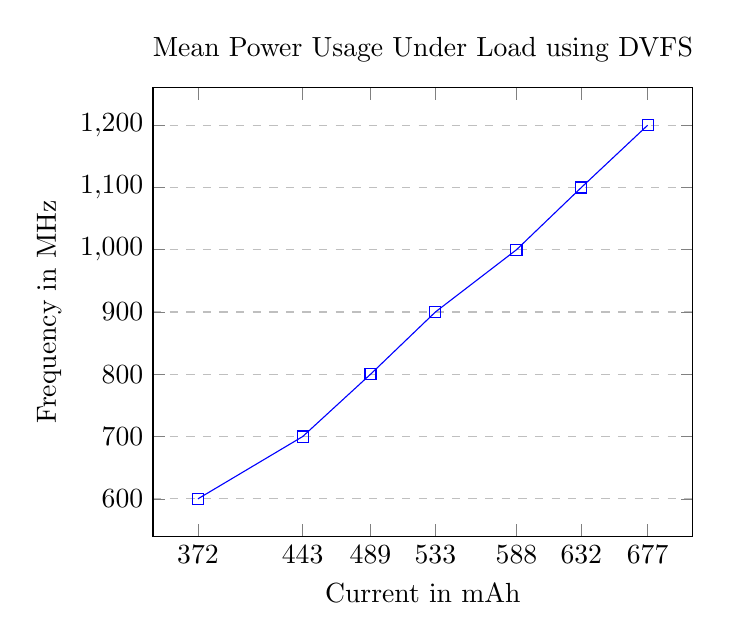
\begin{tikzpicture}
    \begin{axis}[
        title={Mean Power Usage Under Load using DVFS},
        xlabel={Current in mAh},
        ylabel={Frequency in MHz},
        ytick=data,
        xtick=data,
        ymajorgrids=true,
        grid style=dashed,
        cycle list name=color list,
    ]
    \addplot[
        color=blue,
        mark=square,
    ]
    coordinates {
        (372,600)
        (443,700)
        (489,800)
        (533,900)
        (588,1000)
        (632,1100)
        (677,1200)
    };
    \end{axis}
\end{tikzpicture}
\hspace{.5cm}

\end{document}

    \caption{Mean power usage under load with different frequencies}
    \label{fig:freq_mean}
\end{figure}


\subsection{Scaling the Output of the PV Modules}

The PV modules utilized in this version of the testbed are also distributed by
SwitchDoc Labs. They state that one panel is capable of generating a peak
current of \mbox{330 mA} at \mbox{6
V}.\footnote{\url{https://switchdoc.com/2016/06/solar-panel-comparison-sunlight-test/}}
However, even while testing under strong sunlight, the modules were only capable
of generating a third of the current that is stated. In figure
\ref{fig:freq_load} it can be observed that four of these PV modules would
roughly only be capable of supplying the necessary current to the Raspberry Pi
clocked at \mbox{400 MHz}, the lowest possible clock frequency. With this
current supplied, there is no margin for adjusting the energy consumption of the
compute node to the production of the PV modules, as the clock speed could never
surpass \mbox{400 MHz}. Therefore to ensure an environment, in which the whole
spectrum of energy consumed by the compute node at different frequencies can be
supplied in theory, measured currents generated by the PV modules are multiplied
by the factor three. Since the currents are still measured and reacted to in
real time, the requirements for a testbed are still met, as presented in section
\ref{sec:testbeds_emulations_and_simulations}.

\subsection{The Approach}

\begin{figure}
    \centering
    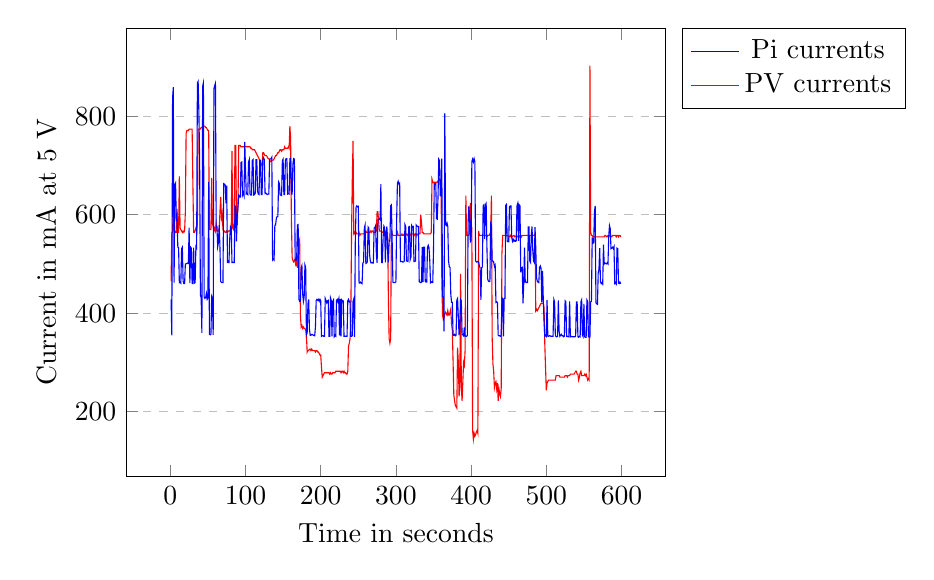
\begin{tikzpicture}
    \begin{axis}[
        xlabel={Time in seconds},
        ylabel={Current in mA at 5 V},
        %ytick=data,
        %xtick=data,
        ymajorgrids=true,
        reverse legend,
        cycle list name=color list,
        legend pos=outer north east,
        grid style=dashed,
    ]
    \addplot
    coordinates {
        (1,465)
        (2,564)
        (3,564)
        (4,618)
        (5,567)
        (6,567)
        (7,564)
        (8,564)
        (9,612)
        (10,564)
        (11,564)
        (12,678)
        (13,573)
        (14,570)
        (15,567)
        (16,564)
        (17,567)
        (18,564)
        (19,567)
        (20,606)
        (21,765)
        (22,771)
        (23,771)
        (24,771)
        (25,774)
        (26,774)
        (27,774)
        (28,774)
        (29,774)
        (30,663)
        (31,564)
        (32,564)
        (33,567)
        (34,573)
        (35,567)
        (36,582)
        (37,774)
        (38,774)
        (39,774)
        (40,774)
        (41,777)
        (42,777)
        (43,780)
        (44,780)
        (45,780)
        (46,780)
        (47,777)
        (48,777)
        (49,774)
        (50,771)
        (51,771)
        (52,570)
        (53,570)
        (54,570)
        (55,675)
        (56,582)
        (57,576)
        (58,567)
        (59,573)
        (60,567)
        (61,582)
        (62,567)
        (63,567)
        (64,567)
        (65,567)
        (66,606)
        (67,636)
        (68,594)
        (69,603)
        (70,570)
        (71,567)
        (72,567)
        (73,564)
        (74,564)
        (75,567)
        (76,564)
        (77,567)
        (78,567)
        (79,567)
        (80,567)
        (81,567)
        (82,729)
        (83,573)
        (84,570)
        (85,567)
        (86,741)
        (87,741)
        (88,591)
        (89,579)
        (90,624)
        (91,741)
        (92,741)
        (93,741)
        (94,738)
        (95,738)
        (96,738)
        (97,738)
        (98,738)
        (99,738)
        (100,738)
        (101,738)
        (102,738)
        (103,738)
        (104,738)
        (105,738)
        (106,738)
        (107,735)
        (108,735)
        (109,732)
        (110,732)
        (111,732)
        (112,732)
        (113,729)
        (114,726)
        (115,723)
        (116,720)
        (117,717)
        (118,714)
        (119,708)
        (120,705)
        (121,702)
        (122,699)
        (123,726)
        (124,726)
        (125,723)
        (126,720)
        (127,720)
        (128,720)
        (129,717)
        (130,714)
        (131,714)
        (132,711)
        (133,708)
        (134,708)
        (135,711)
        (136,711)
        (137,711)
        (138,714)
        (139,717)
        (140,720)
        (141,720)
        (142,723)
        (143,726)
        (144,726)
        (145,729)
        (146,732)
        (147,732)
        (148,729)
        (149,732)
        (150,732)
        (151,732)
        (152,738)
        (153,735)
        (154,735)
        (155,735)
        (156,735)
        (157,738)
        (158,735)
        (159,780)
        (160,753)
        (161,591)
        (162,513)
        (163,507)
        (164,504)
        (165,507)
        (166,510)
        (167,495)
        (168,519)
        (169,492)
        (170,510)
        (171,543)
        (172,549)
        (173,396)
        (174,372)
        (175,375)
        (176,369)
        (177,372)
        (178,369)
        (179,369)
        (180,366)
        (181,354)
        (182,321)
        (183,324)
        (184,324)
        (185,327)
        (186,327)
        (187,324)
        (188,327)
        (189,324)
        (190,324)
        (191,324)
        (192,324)
        (193,321)
        (194,324)
        (195,324)
        (196,321)
        (197,321)
        (198,318)
        (199,315)
        (200,315)
        (201,291)
        (202,270)
        (203,273)
        (204,276)
        (205,279)
        (206,279)
        (207,279)
        (208,279)
        (209,279)
        (210,279)
        (211,279)
        (212,276)
        (213,279)
        (214,276)
        (215,276)
        (216,279)
        (217,279)
        (218,279)
        (219,279)
        (220,282)
        (221,282)
        (222,282)
        (223,282)
        (224,282)
        (225,282)
        (226,282)
        (227,279)
        (228,282)
        (229,282)
        (230,279)
        (231,282)
        (232,279)
        (233,279)
        (234,276)
        (235,276)
        (236,282)
        (237,333)
        (238,339)
        (239,348)
        (240,387)
        (241,564)
        (242,672)
        (243,750)
        (244,561)
        (245,564)
        (246,561)
        (247,564)
        (248,561)
        (249,561)
        (250,561)
        (251,564)
        (252,558)
        (253,561)
        (254,561)
        (255,561)
        (256,561)
        (257,561)
        (258,561)
        (259,564)
        (260,567)
        (261,564)
        (262,564)
        (263,564)
        (264,564)
        (265,564)
        (266,567)
        (267,564)
        (268,567)
        (269,567)
        (270,564)
        (271,564)
        (272,564)
        (273,567)
        (274,567)
        (275,606)
        (276,606)
        (277,588)
        (278,567)
        (279,567)
        (280,567)
        (281,567)
        (282,564)
        (283,564)
        (284,564)
        (285,558)
        (286,561)
        (287,561)
        (288,564)
        (289,564)
        (290,429)
        (291,348)
        (292,339)
        (293,348)
        (294,567)
        (295,561)
        (296,558)
        (297,558)
        (298,558)
        (299,558)
        (300,558)
        (301,558)
        (302,564)
        (303,558)
        (304,558)
        (305,558)
        (306,558)
        (307,558)
        (308,561)
        (309,558)
        (310,558)
        (311,561)
        (312,558)
        (313,561)
        (314,561)
        (315,558)
        (316,561)
        (317,561)
        (318,561)
        (319,558)
        (320,561)
        (321,561)
        (322,561)
        (323,561)
        (324,561)
        (325,558)
        (326,561)
        (327,561)
        (328,558)
        (329,561)
        (330,561)
        (331,561)
        (332,561)
        (333,600)
        (334,585)
        (335,564)
        (336,564)
        (337,561)
        (338,561)
        (339,561)
        (340,561)
        (341,561)
        (342,561)
        (343,561)
        (344,561)
        (345,561)
        (346,561)
        (347,564)
        (348,672)
        (349,666)
        (350,666)
        (351,666)
        (352,666)
        (353,666)
        (354,666)
        (355,666)
        (356,669)
        (357,669)
        (358,672)
        (359,669)
        (360,672)
        (361,474)
        (362,396)
        (363,387)
        (364,390)
        (365,399)
        (366,402)
        (367,399)
        (368,396)
        (369,405)
        (370,396)
        (371,396)
        (372,402)
        (373,408)
        (374,378)
        (375,366)
        (376,303)
        (377,234)
        (378,222)
        (379,213)
        (380,210)
        (381,207)
        (382,330)
        (383,300)
        (384,231)
        (385,252)
        (386,480)
        (387,249)
        (388,222)
        (389,261)
        (390,300)
        (391,294)
        (392,324)
        (393,639)
        (394,558)
        (395,558)
        (396,558)
        (397,558)
        (398,564)
        (399,624)
        (400,561)
        (401,567)
        (402,162)
        (403,144)
        (404,156)
        (405,150)
        (406,153)
        (407,159)
        (408,162)
        (409,156)
        (410,567)
        (411,558)
        (412,558)
        (413,558)
        (414,558)
        (415,558)
        (416,558)
        (417,558)
        (418,558)
        (419,558)
        (420,558)
        (421,555)
        (422,558)
        (423,558)
        (424,558)
        (425,561)
        (426,558)
        (427,639)
        (428,351)
        (429,297)
        (430,282)
        (431,249)
        (432,258)
        (433,261)
        (434,246)
        (435,258)
        (436,222)
        (437,246)
        (438,237)
        (439,231)
        (440,246)
        (441,522)
        (442,558)
        (443,558)
        (444,558)
        (445,558)
        (446,558)
        (447,558)
        (448,558)
        (449,558)
        (450,555)
        (451,555)
        (452,558)
        (453,555)
        (454,555)
        (455,555)
        (456,558)
        (457,558)
        (458,555)
        (459,555)
        (460,558)
        (461,555)
        (462,555)
        (463,558)
        (464,555)
        (465,558)
        (466,558)
        (467,555)
        (468,558)
        (469,558)
        (470,558)
        (471,558)
        (472,558)
        (473,558)
        (474,558)
        (475,558)
        (476,558)
        (477,558)
        (478,558)
        (479,558)
        (480,558)
        (481,558)
        (482,558)
        (483,558)
        (484,558)
        (485,561)
        (486,405)
        (487,408)
        (488,405)
        (489,408)
        (490,411)
        (491,414)
        (492,417)
        (493,420)
        (494,420)
        (495,420)
        (496,420)
        (497,411)
        (498,336)
        (499,288)
        (500,243)
        (501,258)
        (502,261)
        (503,264)
        (504,264)
        (505,264)
        (506,264)
        (507,264)
        (508,264)
        (509,264)
        (510,264)
        (511,264)
        (512,264)
        (513,273)
        (514,273)
        (515,273)
        (516,273)
        (517,273)
        (518,270)
        (519,270)
        (520,270)
        (521,270)
        (522,270)
        (523,270)
        (524,270)
        (525,273)
        (526,273)
        (527,273)
        (528,270)
        (529,273)
        (530,273)
        (531,273)
        (532,276)
        (533,276)
        (534,276)
        (535,276)
        (536,276)
        (537,276)
        (538,279)
        (539,282)
        (540,282)
        (541,276)
        (542,276)
        (543,264)
        (544,270)
        (545,279)
        (546,282)
        (547,273)
        (548,273)
        (549,273)
        (550,273)
        (551,276)
        (552,273)
        (553,276)
        (554,270)
        (555,264)
        (556,267)
        (557,264)
        (558,903)
        (559,564)
        (560,558)
        (561,558)
        (562,555)
        (563,555)
        (564,555)
        (565,555)
        (566,555)
        (567,555)
        (568,555)
        (569,555)
        (570,555)
        (571,555)
        (572,555)
        (573,555)
        (574,555)
        (575,555)
        (576,555)
        (577,555)
        (578,558)
        (579,558)
        (580,555)
        (581,555)
        (582,558)
        (583,558)
        (584,558)
        (585,558)
        (586,555)
        (587,555)
        (588,558)
        (589,558)
        (590,558)
        (591,558)
        (592,558)
        (593,555)
        (594,558)
        (595,558)
        (596,555)
        (597,558)
        (598,558)
        (599,555)
    };
    \addlegendentry{PV currents}
    \addplot
    coordinates {
        (1,428)
        (2,355)
        (3,837)
        (4,859)
        (5,462)
        (6,660)
        (7,664)
        (8,589)
        (9,590)
        (10,534)
        (11,533)
        (12,462)
        (13,463)
        (14,461)
        (15,531)
        (16,534)
        (17,465)
        (18,460)
        (19,460)
        (20,500)
        (21,500)
        (22,501)
        (23,502)
        (24,501)
        (25,574)
        (26,461)
        (27,534)
        (28,532)
        (29,460)
        (30,460)
        (31,533)
        (32,461)
        (33,462)
        (34,535)
        (35,532)
        (36,868)
        (37,871)
        (38,807)
        (39,709)
        (40,437)
        (41,431)
        (42,360)
        (43,861)
        (44,868)
        (45,433)
        (46,430)
        (47,432)
        (48,440)
        (49,428)
        (50,431)
        (51,667)
        (52,357)
        (53,356)
        (54,357)
        (55,433)
        (56,428)
        (57,356)
        (58,856)
        (59,862)
        (60,867)
        (61,575)
        (62,576)
        (63,535)
        (64,544)
        (65,579)
        (66,534)
        (67,465)
        (68,462)
        (69,462)
        (70,462)
        (71,663)
        (72,662)
        (73,660)
        (74,623)
        (75,659)
        (76,503)
        (77,503)
        (78,503)
        (79,551)
        (80,576)
        (81,574)
        (82,503)
        (83,503)
        (84,503)
        (85,503)
        (86,618)
        (87,616)
        (88,546)
        (89,600)
        (90,616)
        (91,639)
        (92,636)
        (93,636)
        (94,706)
        (95,707)
        (96,640)
        (97,645)
        (98,639)
        (99,748)
        (100,692)
        (101,642)
        (102,643)
        (103,641)
        (104,707)
        (105,712)
        (106,642)
        (107,640)
        (108,640)
        (109,710)
        (110,712)
        (111,640)
        (112,641)
        (113,644)
        (114,712)
        (115,712)
        (116,648)
        (117,642)
        (118,641)
        (119,711)
        (120,711)
        (121,641)
        (122,641)
        (123,711)
        (124,716)
        (125,712)
        (126,643)
        (127,644)
        (128,642)
        (129,641)
        (130,642)
        (131,642)
        (132,713)
        (133,713)
        (134,714)
        (135,717)
        (136,508)
        (137,510)
        (138,508)
        (139,579)
        (140,579)
        (141,593)
        (142,596)
        (143,596)
        (144,667)
        (145,664)
        (146,640)
        (147,640)
        (148,639)
        (149,710)
        (150,713)
        (151,641)
        (152,641)
        (153,710)
        (154,714)
        (155,714)
        (156,642)
        (157,643)
        (158,642)
        (159,714)
        (160,715)
        (161,642)
        (162,642)
        (163,702)
        (164,714)
        (165,713)
        (166,508)
        (167,508)
        (168,508)
        (169,579)
        (170,580)
        (171,428)
        (172,424)
        (173,424)
        (174,493)
        (175,497)
        (176,439)
        (177,424)
        (178,433)
        (179,498)
        (180,493)
        (181,356)
        (182,360)
        (183,419)
        (184,428)
        (185,368)
        (186,355)
        (187,355)
        (188,357)
        (189,357)
        (190,355)
        (191,355)
        (192,354)
        (193,373)
        (194,426)
        (195,428)
        (196,426)
        (197,428)
        (198,424)
        (199,428)
        (200,425)
        (201,353)
        (202,354)
        (203,354)
        (204,353)
        (205,353)
        (206,430)
        (207,426)
        (208,421)
        (209,425)
        (210,426)
        (211,353)
        (212,353)
        (213,431)
        (214,426)
        (215,353)
        (216,424)
        (217,427)
        (218,352)
        (219,354)
        (220,353)
        (221,426)
        (222,428)
        (223,423)
        (224,429)
        (225,355)
        (226,429)
        (227,353)
        (228,427)
        (229,425)
        (230,425)
        (231,353)
        (232,353)
        (233,353)
        (234,353)
        (235,353)
        (236,425)
        (237,428)
        (238,423)
        (239,424)
        (240,353)
        (241,353)
        (242,354)
        (243,424)
        (244,429)
        (245,352)
        (246,546)
        (247,615)
        (248,618)
        (249,616)
        (250,617)
        (251,461)
        (252,461)
        (253,463)
        (254,461)
        (255,460)
        (256,502)
        (257,503)
        (258,573)
        (259,579)
        (260,501)
        (261,502)
        (262,504)
        (263,575)
        (264,573)
        (265,519)
        (266,506)
        (267,502)
        (268,503)
        (269,502)
        (270,502)
        (271,573)
        (272,574)
        (273,578)
        (274,519)
        (275,502)
        (276,590)
        (277,590)
        (278,592)
        (279,590)
        (280,662)
        (281,503)
        (282,503)
        (283,555)
        (284,577)
        (285,574)
        (286,503)
        (287,563)
        (288,576)
        (289,525)
        (290,503)
        (291,548)
        (292,547)
        (293,618)
        (294,620)
        (295,548)
        (296,463)
        (297,462)
        (298,462)
        (299,463)
        (300,463)
        (301,591)
        (302,664)
        (303,668)
        (304,662)
        (305,664)
        (306,505)
        (307,505)
        (308,505)
        (309,504)
        (310,504)
        (311,505)
        (312,580)
        (313,576)
        (314,506)
        (315,506)
        (316,505)
        (317,575)
        (318,576)
        (319,509)
        (320,514)
        (321,578)
        (322,575)
        (323,576)
        (324,505)
        (325,505)
        (326,506)
        (327,579)
        (328,577)
        (329,576)
        (330,576)
        (331,464)
        (332,463)
        (333,462)
        (334,463)
        (335,534)
        (336,463)
        (337,534)
        (338,534)
        (339,465)
        (340,463)
        (341,463)
        (342,534)
        (343,538)
        (344,533)
        (345,508)
        (346,462)
        (347,464)
        (348,462)
        (349,462)
        (350,529)
        (351,663)
        (352,663)
        (353,663)
        (354,592)
        (355,591)
        (356,636)
        (357,713)
        (358,710)
        (359,639)
        (360,638)
        (361,714)
        (362,433)
        (363,433)
        (364,363)
        (365,806)
        (366,580)
        (367,578)
        (368,583)
        (369,576)
        (370,506)
        (371,494)
        (372,493)
        (373,438)
        (374,422)
        (375,422)
        (376,355)
        (377,355)
        (378,357)
        (379,354)
        (380,355)
        (381,427)
        (382,430)
        (383,392)
        (384,355)
        (385,371)
        (386,428)
        (387,425)
        (388,357)
        (389,356)
        (390,354)
        (391,371)
        (392,353)
        (393,353)
        (394,353)
        (395,355)
        (396,582)
        (397,618)
        (398,597)
        (399,545)
        (400,547)
        (401,708)
        (402,713)
        (403,707)
        (404,714)
        (405,708)
        (406,506)
        (407,504)
        (408,504)
        (409,505)
        (410,504)
        (411,496)
        (412,492)
        (413,427)
        (414,492)
        (415,494)
        (416,618)
        (417,620)
        (418,551)
        (419,620)
        (420,623)
        (421,536)
        (422,470)
        (423,465)
        (424,464)
        (425,464)
        (426,582)
        (427,578)
        (428,506)
        (429,506)
        (430,504)
        (431,495)
        (432,498)
        (433,422)
        (434,423)
        (435,422)
        (436,355)
        (437,354)
        (438,354)
        (439,353)
        (440,356)
        (441,431)
        (442,429)
        (443,353)
        (444,430)
        (445,430)
        (446,619)
        (447,621)
        (448,546)
        (449,545)
        (450,545)
        (451,616)
        (452,618)
        (453,618)
        (454,554)
        (455,546)
        (456,550)
        (457,546)
        (458,548)
        (459,546)
        (460,547)
        (461,618)
        (462,623)
        (463,547)
        (464,620)
        (465,618)
        (466,483)
        (467,492)
        (468,493)
        (469,420)
        (470,461)
        (471,533)
        (472,463)
        (473,463)
        (474,462)
        (475,462)
        (476,575)
        (477,575)
        (478,506)
        (479,503)
        (480,558)
        (481,576)
        (482,528)
        (483,506)
        (484,503)
        (485,575)
        (486,532)
        (487,472)
        (488,465)
        (489,463)
        (490,462)
        (491,493)
        (492,496)
        (493,491)
        (494,422)
        (495,486)
        (496,427)
        (497,383)
        (498,353)
        (499,355)
        (500,353)
        (501,427)
        (502,353)
        (503,353)
        (504,354)
        (505,354)
        (506,353)
        (507,353)
        (508,353)
        (509,353)
        (510,428)
        (511,423)
        (512,356)
        (513,352)
        (514,352)
        (515,353)
        (516,426)
        (517,364)
        (518,353)
        (519,355)
        (520,357)
        (521,354)
        (522,354)
        (523,352)
        (524,353)
        (525,425)
        (526,423)
        (527,353)
        (528,353)
        (529,352)
        (530,352)
        (531,424)
        (532,352)
        (533,353)
        (534,352)
        (535,352)
        (536,352)
        (537,352)
        (538,352)
        (539,353)
        (540,423)
        (541,423)
        (542,352)
        (543,351)
        (544,353)
        (545,352)
        (546,423)
        (547,427)
        (548,355)
        (549,352)
        (550,419)
        (551,352)
        (552,351)
        (553,351)
        (554,427)
        (555,424)
        (556,352)
        (557,352)
        (558,351)
        (559,423)
        (560,424)
        (561,554)
        (562,542)
        (563,543)
        (564,606)
        (565,618)
        (566,421)
        (567,419)
        (568,418)
        (569,481)
        (570,489)
        (571,532)
        (572,464)
        (573,460)
        (574,462)
        (575,459)
        (576,539)
        (577,500)
        (578,502)
        (579,501)
        (580,500)
        (581,502)
        (582,500)
        (583,556)
        (584,578)
        (585,572)
        (586,531)
        (587,532)
        (588,534)
        (589,531)
        (590,535)
        (591,460)
        (592,461)
        (593,459)
        (594,532)
        (595,531)
        (596,461)
        (597,460)
        (598,463)
        (599,460)
    };
    \addlegendentry{Pi currents}
    \end{axis}
\end{tikzpicture}

    \caption{aware}
    \label{fig:aware}
\end{figure}

\begin{figure}
    \centering
    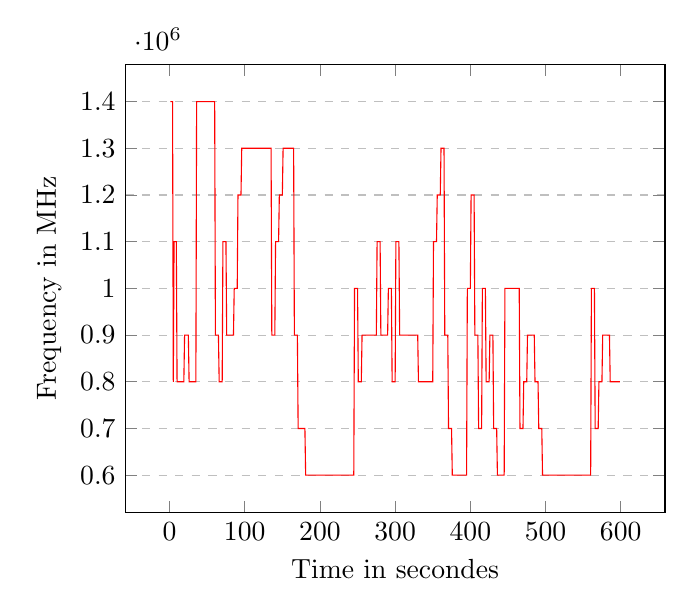
\begin{tikzpicture}
    \begin{axis}[
        xlabel={Time in secondes},
        ylabel={Frequency in MHz},
        ytick=data,
        %xtick=data,
        ymajorgrids=true,
        grid style=dashed,
        legend pos=outer north east,
        cycle list name=color list,
    ]
    \addplot
    coordinates {
        (1,1400000)
        (2,1400000)
        (3,1400000)
        (4,1400000)
        (5,800000)
        (6,1100000)
        (7,1100000)
        (8,1100000)
        (9,1100000)
        (10,800000)
        (11,800000)
        (12,800000)
        (13,800000)
        (14,800000)
        (15,800000)
        (16,800000)
        (17,800000)
        (18,800000)
        (19,800000)
        (20,900000)
        (21,900000)
        (22,900000)
        (23,900000)
        (24,900000)
        (25,900000)
        (26,800000)
        (27,800000)
        (28,800000)
        (29,800000)
        (30,800000)
        (31,800000)
        (32,800000)
        (33,800000)
        (34,800000)
        (35,800000)
        (36,1400000)
        (37,1400000)
        (38,1400000)
        (39,1400000)
        (40,1400000)
        (41,1400000)
        (42,1400000)
        (43,1400000)
        (44,1400000)
        (45,1400000)
        (46,1400000)
        (47,1400000)
        (48,1400000)
        (49,1400000)
        (50,1400000)
        (51,1400000)
        (52,1400000)
        (53,1400000)
        (54,1400000)
        (55,1400000)
        (56,1400000)
        (57,1400000)
        (58,1400000)
        (59,1400000)
        (60,1400000)
        (61,900000)
        (62,900000)
        (63,900000)
        (64,900000)
        (65,900000)
        (66,800000)
        (67,800000)
        (68,800000)
        (69,800000)
        (70,800000)
        (71,1100000)
        (72,1100000)
        (73,1100000)
        (74,1100000)
        (75,1100000)
        (76,900000)
        (77,900000)
        (78,900000)
        (79,900000)
        (80,900000)
        (81,900000)
        (82,900000)
        (83,900000)
        (84,900000)
        (85,900000)
        (86,1000000)
        (87,1000000)
        (88,1000000)
        (89,1000000)
        (90,1000000)
        (91,1200000)
        (92,1200000)
        (93,1200000)
        (94,1200000)
        (95,1200000)
        (96,1300000)
        (97,1300000)
        (98,1300000)
        (99,1300000)
        (100,1300000)
        (101,1300000)
        (102,1300000)
        (103,1300000)
        (104,1300000)
        (105,1300000)
        (106,1300000)
        (107,1300000)
        (108,1300000)
        (109,1300000)
        (110,1300000)
        (111,1300000)
        (112,1300000)
        (113,1300000)
        (114,1300000)
        (115,1300000)
        (116,1300000)
        (117,1300000)
        (118,1300000)
        (119,1300000)
        (120,1300000)
        (121,1300000)
        (122,1300000)
        (123,1300000)
        (124,1300000)
        (125,1300000)
        (126,1300000)
        (127,1300000)
        (128,1300000)
        (129,1300000)
        (130,1300000)
        (131,1300000)
        (132,1300000)
        (133,1300000)
        (134,1300000)
        (135,1300000)
        (136,900000)
        (137,900000)
        (138,900000)
        (139,900000)
        (140,900000)
        (141,1100000)
        (142,1100000)
        (143,1100000)
        (144,1100000)
        (145,1100000)
        (146,1200000)
        (147,1200000)
        (148,1200000)
        (149,1200000)
        (150,1200000)
        (151,1300000)
        (152,1300000)
        (153,1300000)
        (154,1300000)
        (155,1300000)
        (156,1300000)
        (157,1300000)
        (158,1300000)
        (159,1300000)
        (160,1300000)
        (161,1300000)
        (162,1300000)
        (163,1300000)
        (164,1300000)
        (165,1300000)
        (166,900000)
        (167,900000)
        (168,900000)
        (169,900000)
        (170,900000)
        (171,700000)
        (172,700000)
        (173,700000)
        (174,700000)
        (175,700000)
        (176,700000)
        (177,700000)
        (178,700000)
        (179,700000)
        (180,700000)
        (181,600000)
        (182,600000)
        (183,600000)
        (184,600000)
        (185,600000)
        (186,600000)
        (187,600000)
        (188,600000)
        (189,600000)
        (190,600000)
        (191,600000)
        (192,600000)
        (193,600000)
        (194,600000)
        (195,600000)
        (196,600000)
        (197,600000)
        (198,600000)
        (199,600000)
        (200,600000)
        (201,600000)
        (202,600000)
        (203,600000)
        (204,600000)
        (205,600000)
        (206,600000)
        (207,600000)
        (208,600000)
        (209,600000)
        (210,600000)
        (211,600000)
        (212,600000)
        (213,600000)
        (214,600000)
        (215,600000)
        (216,600000)
        (217,600000)
        (218,600000)
        (219,600000)
        (220,600000)
        (221,600000)
        (222,600000)
        (223,600000)
        (224,600000)
        (225,600000)
        (226,600000)
        (227,600000)
        (228,600000)
        (229,600000)
        (230,600000)
        (231,600000)
        (232,600000)
        (233,600000)
        (234,600000)
        (235,600000)
        (236,600000)
        (237,600000)
        (238,600000)
        (239,600000)
        (240,600000)
        (241,600000)
        (242,600000)
        (243,600000)
        (244,600000)
        (245,600000)
        (246,1000000)
        (247,1000000)
        (248,1000000)
        (249,1000000)
        (250,1000000)
        (251,800000)
        (252,800000)
        (253,800000)
        (254,800000)
        (255,800000)
        (256,900000)
        (257,900000)
        (258,900000)
        (259,900000)
        (260,900000)
        (261,900000)
        (262,900000)
        (263,900000)
        (264,900000)
        (265,900000)
        (266,900000)
        (267,900000)
        (268,900000)
        (269,900000)
        (270,900000)
        (271,900000)
        (272,900000)
        (273,900000)
        (274,900000)
        (275,900000)
        (276,1100000)
        (277,1100000)
        (278,1100000)
        (279,1100000)
        (280,1100000)
        (281,900000)
        (282,900000)
        (283,900000)
        (284,900000)
        (285,900000)
        (286,900000)
        (287,900000)
        (288,900000)
        (289,900000)
        (290,900000)
        (291,1000000)
        (292,1000000)
        (293,1000000)
        (294,1000000)
        (295,1000000)
        (296,800000)
        (297,800000)
        (298,800000)
        (299,800000)
        (300,800000)
        (301,1100000)
        (302,1100000)
        (303,1100000)
        (304,1100000)
        (305,1100000)
        (306,900000)
        (307,900000)
        (308,900000)
        (309,900000)
        (310,900000)
        (311,900000)
        (312,900000)
        (313,900000)
        (314,900000)
        (315,900000)
        (316,900000)
        (317,900000)
        (318,900000)
        (319,900000)
        (320,900000)
        (321,900000)
        (322,900000)
        (323,900000)
        (324,900000)
        (325,900000)
        (326,900000)
        (327,900000)
        (328,900000)
        (329,900000)
        (330,900000)
        (331,800000)
        (332,800000)
        (333,800000)
        (334,800000)
        (335,800000)
        (336,800000)
        (337,800000)
        (338,800000)
        (339,800000)
        (340,800000)
        (341,800000)
        (342,800000)
        (343,800000)
        (344,800000)
        (345,800000)
        (346,800000)
        (347,800000)
        (348,800000)
        (349,800000)
        (350,800000)
        (351,1100000)
        (352,1100000)
        (353,1100000)
        (354,1100000)
        (355,1100000)
        (356,1200000)
        (357,1200000)
        (358,1200000)
        (359,1200000)
        (360,1200000)
        (361,1300000)
        (362,1300000)
        (363,1300000)
        (364,1300000)
        (365,1300000)
        (366,900000)
        (367,900000)
        (368,900000)
        (369,900000)
        (370,900000)
        (371,700000)
        (372,700000)
        (373,700000)
        (374,700000)
        (375,700000)
        (376,600000)
        (377,600000)
        (378,600000)
        (379,600000)
        (380,600000)
        (381,600000)
        (382,600000)
        (383,600000)
        (384,600000)
        (385,600000)
        (386,600000)
        (387,600000)
        (388,600000)
        (389,600000)
        (390,600000)
        (391,600000)
        (392,600000)
        (393,600000)
        (394,600000)
        (395,600000)
        (396,1000000)
        (397,1000000)
        (398,1000000)
        (399,1000000)
        (400,1000000)
        (401,1200000)
        (402,1200000)
        (403,1200000)
        (404,1200000)
        (405,1200000)
        (406,900000)
        (407,900000)
        (408,900000)
        (409,900000)
        (410,900000)
        (411,700000)
        (412,700000)
        (413,700000)
        (414,700000)
        (415,700000)
        (416,1000000)
        (417,1000000)
        (418,1000000)
        (419,1000000)
        (420,1000000)
        (421,800000)
        (422,800000)
        (423,800000)
        (424,800000)
        (425,800000)
        (426,900000)
        (427,900000)
        (428,900000)
        (429,900000)
        (430,900000)
        (431,700000)
        (432,700000)
        (433,700000)
        (434,700000)
        (435,700000)
        (436,600000)
        (437,600000)
        (438,600000)
        (439,600000)
        (440,600000)
        (441,600000)
        (442,600000)
        (443,600000)
        (444,600000)
        (445,600000)
        (446,1000000)
        (447,1000000)
        (448,1000000)
        (449,1000000)
        (450,1000000)
        (451,1000000)
        (452,1000000)
        (453,1000000)
        (454,1000000)
        (455,1000000)
        (456,1000000)
        (457,1000000)
        (458,1000000)
        (459,1000000)
        (460,1000000)
        (461,1000000)
        (462,1000000)
        (463,1000000)
        (464,1000000)
        (465,1000000)
        (466,700000)
        (467,700000)
        (468,700000)
        (469,700000)
        (470,700000)
        (471,800000)
        (472,800000)
        (473,800000)
        (474,800000)
        (475,800000)
        (476,900000)
        (477,900000)
        (478,900000)
        (479,900000)
        (480,900000)
        (481,900000)
        (482,900000)
        (483,900000)
        (484,900000)
        (485,900000)
        (486,800000)
        (487,800000)
        (488,800000)
        (489,800000)
        (490,800000)
        (491,700000)
        (492,700000)
        (493,700000)
        (494,700000)
        (495,700000)
        (496,600000)
        (497,600000)
        (498,600000)
        (499,600000)
        (500,600000)
        (501,600000)
        (502,600000)
        (503,600000)
        (504,600000)
        (505,600000)
        (506,600000)
        (507,600000)
        (508,600000)
        (509,600000)
        (510,600000)
        (511,600000)
        (512,600000)
        (513,600000)
        (514,600000)
        (515,600000)
        (516,600000)
        (517,600000)
        (518,600000)
        (519,600000)
        (520,600000)
        (521,600000)
        (522,600000)
        (523,600000)
        (524,600000)
        (525,600000)
        (526,600000)
        (527,600000)
        (528,600000)
        (529,600000)
        (530,600000)
        (531,600000)
        (532,600000)
        (533,600000)
        (534,600000)
        (535,600000)
        (536,600000)
        (537,600000)
        (538,600000)
        (539,600000)
        (540,600000)
        (541,600000)
        (542,600000)
        (543,600000)
        (544,600000)
        (545,600000)
        (546,600000)
        (547,600000)
        (548,600000)
        (549,600000)
        (550,600000)
        (551,600000)
        (552,600000)
        (553,600000)
        (554,600000)
        (555,600000)
        (556,600000)
        (557,600000)
        (558,600000)
        (559,600000)
        (560,600000)
        (561,1000000)
        (562,1000000)
        (563,1000000)
        (564,1000000)
        (565,1000000)
        (566,700000)
        (567,700000)
        (568,700000)
        (569,700000)
        (570,700000)
        (571,800000)
        (572,800000)
        (573,800000)
        (574,800000)
        (575,800000)
        (576,900000)
        (577,900000)
        (578,900000)
        (579,900000)
        (580,900000)
        (581,900000)
        (582,900000)
        (583,900000)
        (584,900000)
        (585,900000)
        (586,800000)
        (587,800000)
        (588,800000)
        (589,800000)
        (590,800000)
        (591,800000)
        (592,800000)
        (593,800000)
        (594,800000)
        (595,800000)
        (596,800000)
        (597,800000)
        (598,800000)
        (599,800000)
    };
    \end{axis}
\end{tikzpicture}

    \caption{aware freqs}
    \label{fig:aware_freqs}
\end{figure}
